\section{引言：模型原生计算需要体系结构}
\label{sec:intro}

大语言模型正在从一种"模型技术"演变为一种"系统技术"。
从GPT-3展示少样本学习能力\cite{brown2020gpt3}，到LLaMA系列推动开放模型生态\cite{llama2023}，再到工具使用\cite{schick2023toolformer}、检索增强\cite{lewis2020rag}、自主Agent\cite{yao2023react}和代码生成系统\cite{openhands_paper_2025,sweagent2024}的快速涌现，研究重心已经从"如何训练更强的模型"，转向"如何把智能组织成稳定、可扩展、可审计的系统"。
这一转变同时正在重塑工程实践本身：工程师的角色正从"逐行编写代码"转向"编排管理多个Agent系统"，整个开发生命周期正在从周级别压缩到小时级别\cite{anthropic2026agenticreport}。
然而，当前实践中的许多核心挑战---内存带宽受限\cite{gholami2024memorywall}、缓存复用效率\cite{kwon2023pagedattention}、上下文管理\cite{memgpt2023}、批处理调度\cite{orca2022}、沙箱与权限控制\cite{ironclaw2025}---并非模型本身的能力问题，而是典型的\emph{系统问题}。

这种系统性转变已在工业实践中产生显著效果。
Rakuten的工程师已使用Claude Code在一个包含1250万行代码的代码库上连续自主运行数小时\cite{anthropic2026agenticreport}；Augment Code的一位企业客户将CTO预估需要4--8个月的项目在2周内完成\cite{anthropic2026agenticreport}。
这些案例表明，模型原生系统面临的挑战已经从理论可能性变为工程现实。

面对这些问题，一条自然的思路浮现：经典计算机体系结构曾用一套成熟的分层抽象解决了类似的复杂性管理问题，那么这套思想能否迁移到模型原生计算系统？

\subsection{一个直接的类比}

这个类比的核心映射关系见表~\ref{tab:analogy-mapping}。

\begin{table}[t]
\centering
\footnotesize
\caption{计算机体系结构与模型原生计算系统的核心类比映射。}
\label{tab:analogy-mapping}
\begin{tabularx}{\textwidth}{>{\raggedright\arraybackslash}p{0.28\textwidth}>{\raggedright\arraybackslash}p{0.28\textwidth}>{\raggedright\arraybackslash}p{0.34\textwidth}}
\toprule
\textbf{经典计算} & \textbf{模型原生计算} & \textbf{共同的本质问题} \\
\midrule
CPU（通用处理器） & LLM推理核心 & 通用计算/推理能力 \\
高速缓存（L1/L2/L3） & KV缓存 & 热数据复用与访存优化 \\
内存 \& 虚拟内存 & 上下文窗口 \& 外部记忆 & 有限容量的地址空间管理 \\
操作系统 & Agent运行时 & 调度、权限、资源管理 \\
I/O总线（PCIe/USB） & MCP/A2A协议 & 标准化的外设/工具接入 \\
应用程序与用户 & Agent应用与领域专家用户 & 将计算能力转化为领域解决方案 \\
\bottomrule
\end{tabularx}
\end{table}

具体而言：（1）大语言模型的推理核心承担通用的语义理解与生成能力，类似于CPU执行通用指令集---不同的模型（如GPT-4、Claude、LLaMA）就像不同的CPU微架构，执行同样的"推理任务"但性能特征各异。（2）KV缓存（Key-Value Cache）在自回归解码过程中复用先前计算过的注意力键值对，避免重复计算，这与CPU高速缓存利用时间局部性复用热点数据的原理完全一致；PagedAttention\cite{kwon2023pagedattention}更是直接借鉴了操作系统分页管理的思想，将KV缓存划分为固定大小的"页"进行按需分配。（3）上下文窗口容量有限（如128K token），但Agent需要访问远超此限制的知识和历史交互，这与物理内存有限但程序需要更大地址空间的问题如出一辙；MemGPT\cite{memgpt2023}因此将"虚拟上下文管理"作为核心抽象，类比操作系统的虚拟内存机制。（4）Codex\cite{openai_codex_overview_2026}、Claude Code\cite{anthropic_claudecode_overview_2026}、OpenHands\cite{openhands_paper_2025}等Agent运行时负责任务分解、工具调度、子Agent管理、沙箱隔离与结果提交，其职责范围越来越接近一个操作系统内核。（5）MCP（Model Context Protocol）\cite{mcp_intro_2026}定义了Agent与外部工具之间的标准化接口，A2A（Agent-to-Agent Protocol）\cite{google_a2a_2025}定义了Agent之间的互操作协议，它们共同扮演着"I/O总线"的角色---MCP类似于垂直总线（如PCIe，连接Agent与工具），A2A类似于水平总线（如网络互连，连接Agent与Agent）\cite{agentprotocols2025}。

2023年，Andrej Karpathy用一句简短的话概括了这一直觉："LLMs are not chatbots, they are the kernel process of a new Operating System"\cite{karpathy2023lmos}。
这一观察之所以引发广泛共鸣，正是因为它抓住了正在发生的事实：围绕大模型的工程问题，越来越像经典计算机系统问题。

\begin{figure}[t]
\centering
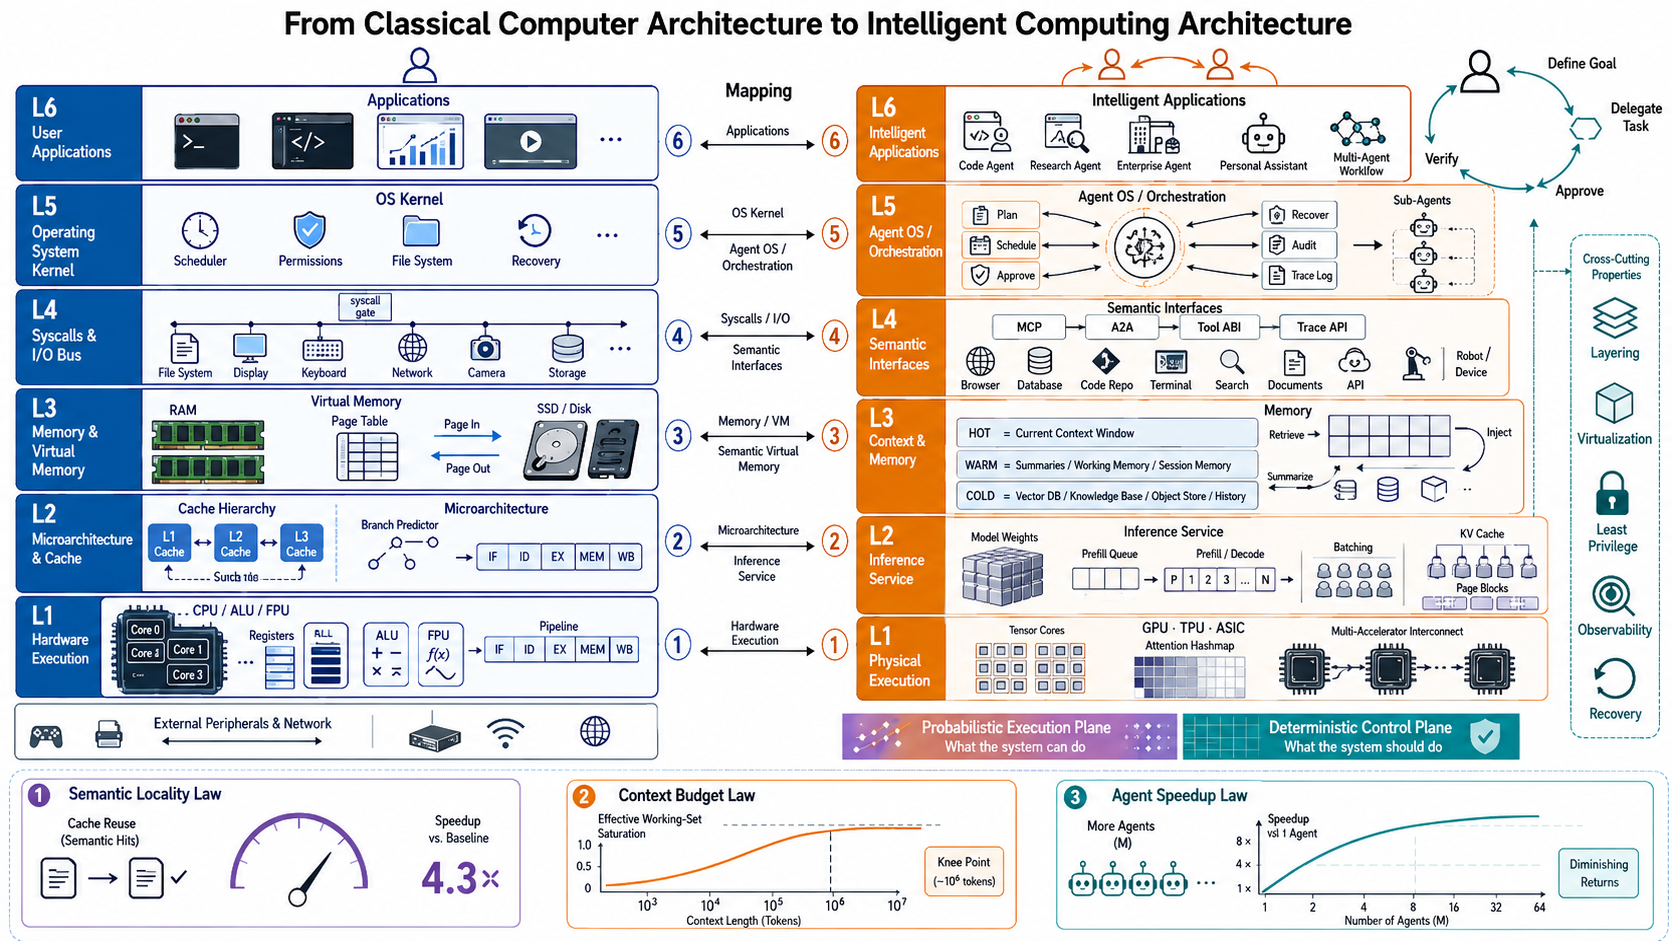
\includegraphics[width=0.98\textwidth]{figures/fig_analogy_map.png}
\caption{计算机体系结构与模型原生计算系统之间的类比映射总览}
\label{fig_analogy_map}
\end{figure}

\subsection{从直觉到问题}

然而，类比本身并不等于理论。"像"不等于"是"。
如果类比仅停留在修辞层面，它只能产生启发性的比喻，不能产生可验证的预测和可操作的设计原则。

近年来，已有多个独立的工作从不同角度触及了这一类比。
AIOS将LLM视为操作系统内核，构建了包含调度器、上下文管理器和内存管理器的Agent运行时\cite{mei2024aios}。
MemGPT用虚拟内存思想管理上下文，提出了"虚拟上下文管理"的抽象\cite{memgpt2023}。
Mi等人从计算机系统演进的角度设计Agent架构，借鉴进程、文件系统等经典概念\cite{mi2025llmagentscomputersystems}。
Ge等人提出"LLM as OS, Agents as Apps"的愿景\cite{ge2023llmos}。
L2MAC将LLM框架称为stored-program automatic computer\cite{holt2024l2mac}。
ArbiterOS把LLM定义为受governor治理的"Probabilistic CPU"\cite{arbiteros2025}。
AgentOS将其视为reasoning kernel\cite{agentos2025}。
MemOS将记忆本身作为操作系统级的一等资源进行管理\cite{memos2025}。
在推理工程侧，Mei等人于2025年系统调研了上下文工程（Context Engineering）这一新兴学科，将其定义为"系统性地优化输入给LLM的全部信息"的工程实践\cite{contextengineer_survey2025}。

这些工作各覆盖了系统栈中的一层或几层---OS层、内存层、Agent内核层、推理层。
但它们之间存在根本性的隐喻冲突：模型到底更像CPU、OS kernel、还是reasoning kernel？
更关键的是，它们之间缺少统一的分层模型、层间接口定义和可量化的设计原则。
此外，这些工作几乎都将人类视为系统的边界条件，而非交互循环的核心组件。
然而最新的工业实证表明，人类判断力与Agent执行能力之间的协作模式---而非Agent的独立能力---才是决定系统效率的关键因素：工程师在工作中约60\%使用AI，但只能"完全委托"0--20\%的任务\cite{anthropic2026agenticreport}；这种"高使用/低委托"的模式也得到了独立研究的印证——开发者平均仅接受约30\%的AI代码建议\cite{dohmke2023seachange}，并且尽管对AI助手的输出存在深深的不信任，仍在广泛使用它们\cite{klemmer2024aiassistants}。
这就是\textbf{协作悖论}：AI已深度嵌入工作流程，但真正有意义的自主委托仍然难以实现。

这一局面与计算机体系结构的早期如出一辙。
在指令集架构（ISA）作为软硬件之间的契约被引入之前，每一代新CPU都需要重写所有软件，每一层的改进都无法被其他层复用。
如果没有类似的契约为模型原生计算服务，每个新系统都必须从零构建，洞见也将在各个项目中孤立存在。

\subsection{本文的贡献}

因此，本文做出以下五项贡献。\emph{核心论点}在于：LLM究竟是CPU还是OS的长期争论，一旦认识到存在两个正交平面——概率执行平面与确定性控制平面——便得以消解；而将这一双平面视角实例化为六层ICA，正是此前任何工作都未曾整合的。

\begin{enumerate}
\item 回到计算机体系结构、操作系统与分布式系统的基本抽象，提炼出适合模型原生系统栈的类比框架，明确类比的适用范围与局限。

\item 系统梳理相关研究工作，揭示现有隐喻之间的冲突，提出\textbf{双平面架构}作为统一解答---将模型原生系统栈划分为\emph{概率执行平面}（模型推理与生成）和\emph{确定性控制平面}（系统调度与控制），两平面通过明确定义的接口交互。

\item 在此基础上提出\textbf{智能计算体系结构（ICA）}---一个六层分层框架，包含层间接口契约与六条设计公理。

\item 提出三条\textbf{Amdahl式设计启发式}---语义局部性、上下文预算与Agent加速比---并用已发表的系统数据\emph{示例说明}其参数取值范围。我们明确指出，这些启发式只是用于整理"信封背面"式直觉的组织工具，而非经过验证的扩展定律：它们将Amdahl定律的解析形式移植到模型原生计算范式，使原本只能定性讨论的设计空间获得可计算的直觉；同时我们将系统性的预测性检验（而非充斥于现有文献的、靠反向求解参数来拟合的那种"检验"）识别为本领域的关键开放问题。

\item 总结当前开源实现和工业实践，给出一个面向未来的研究路线图。
\end{enumerate}

%% ============================================================
